\begin{figure}[htb]
\centering
%\subfloat[side view]{
%	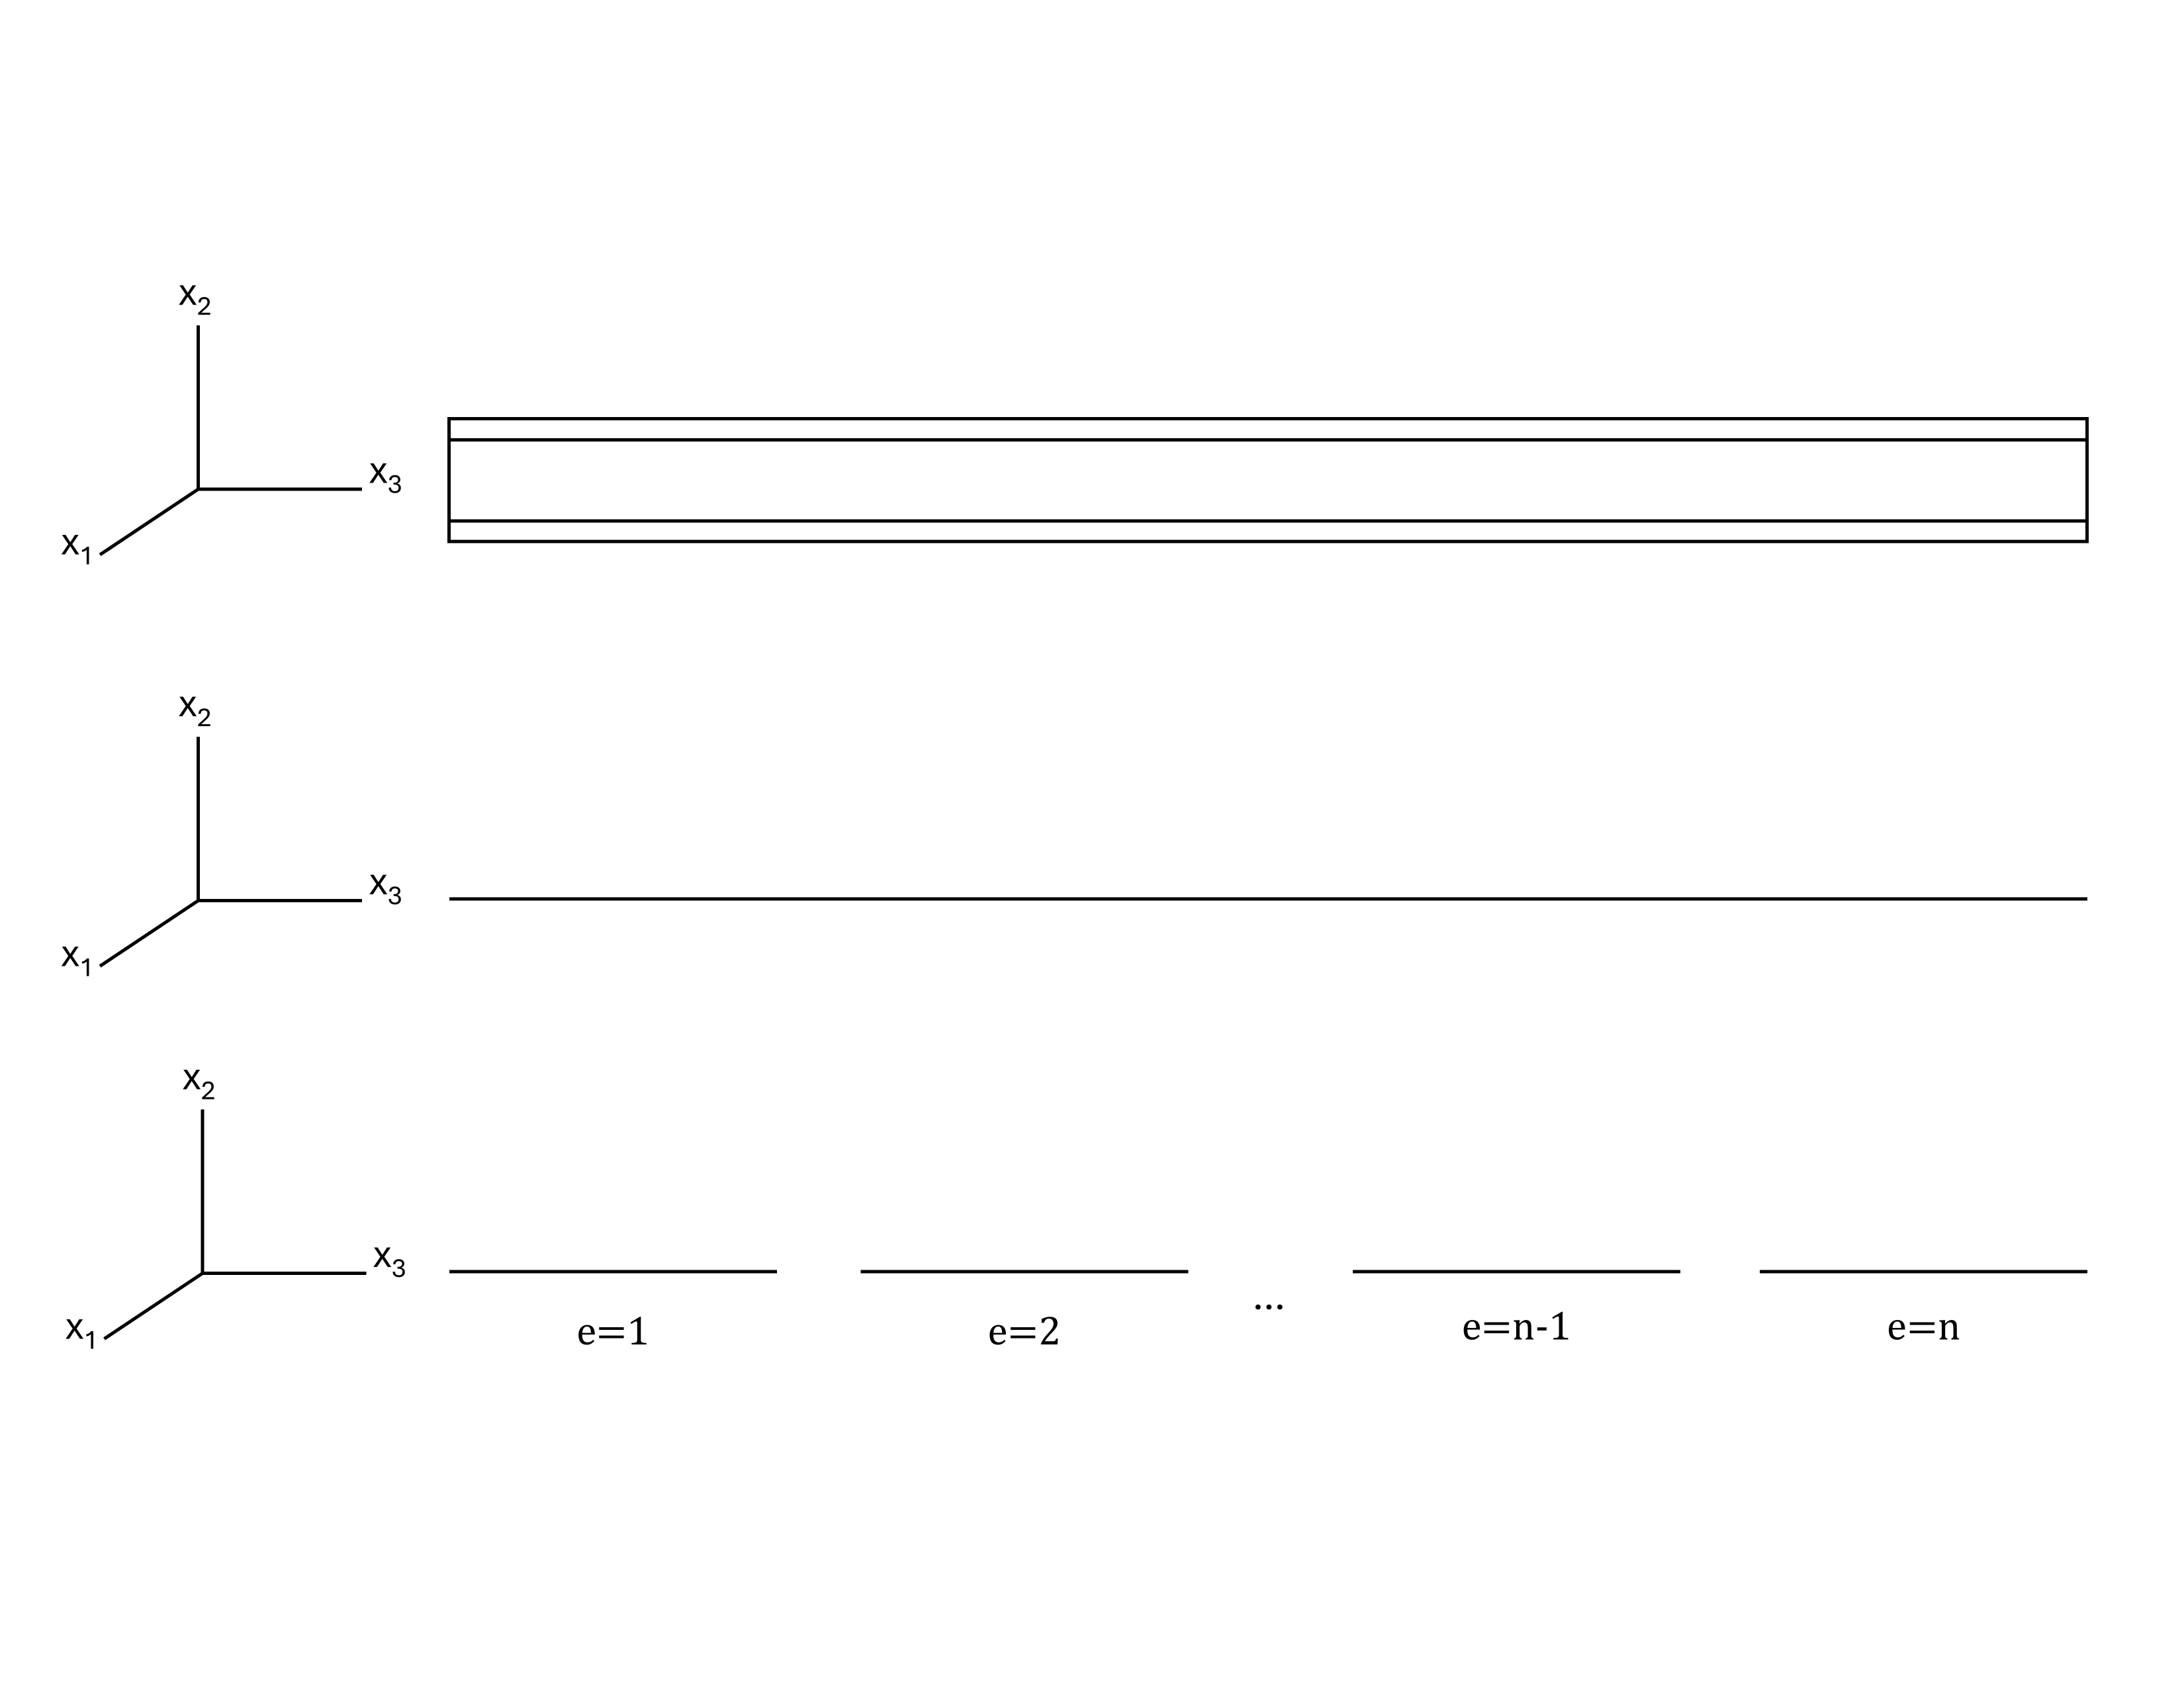
\includegraphics[width=0.7\columnwidth,trim=5.25cm 13cm 0cm 0cm, clip]{figs/beam_to_elements.png}
%}
%\centering
%\subfloat[isometric view]{
%	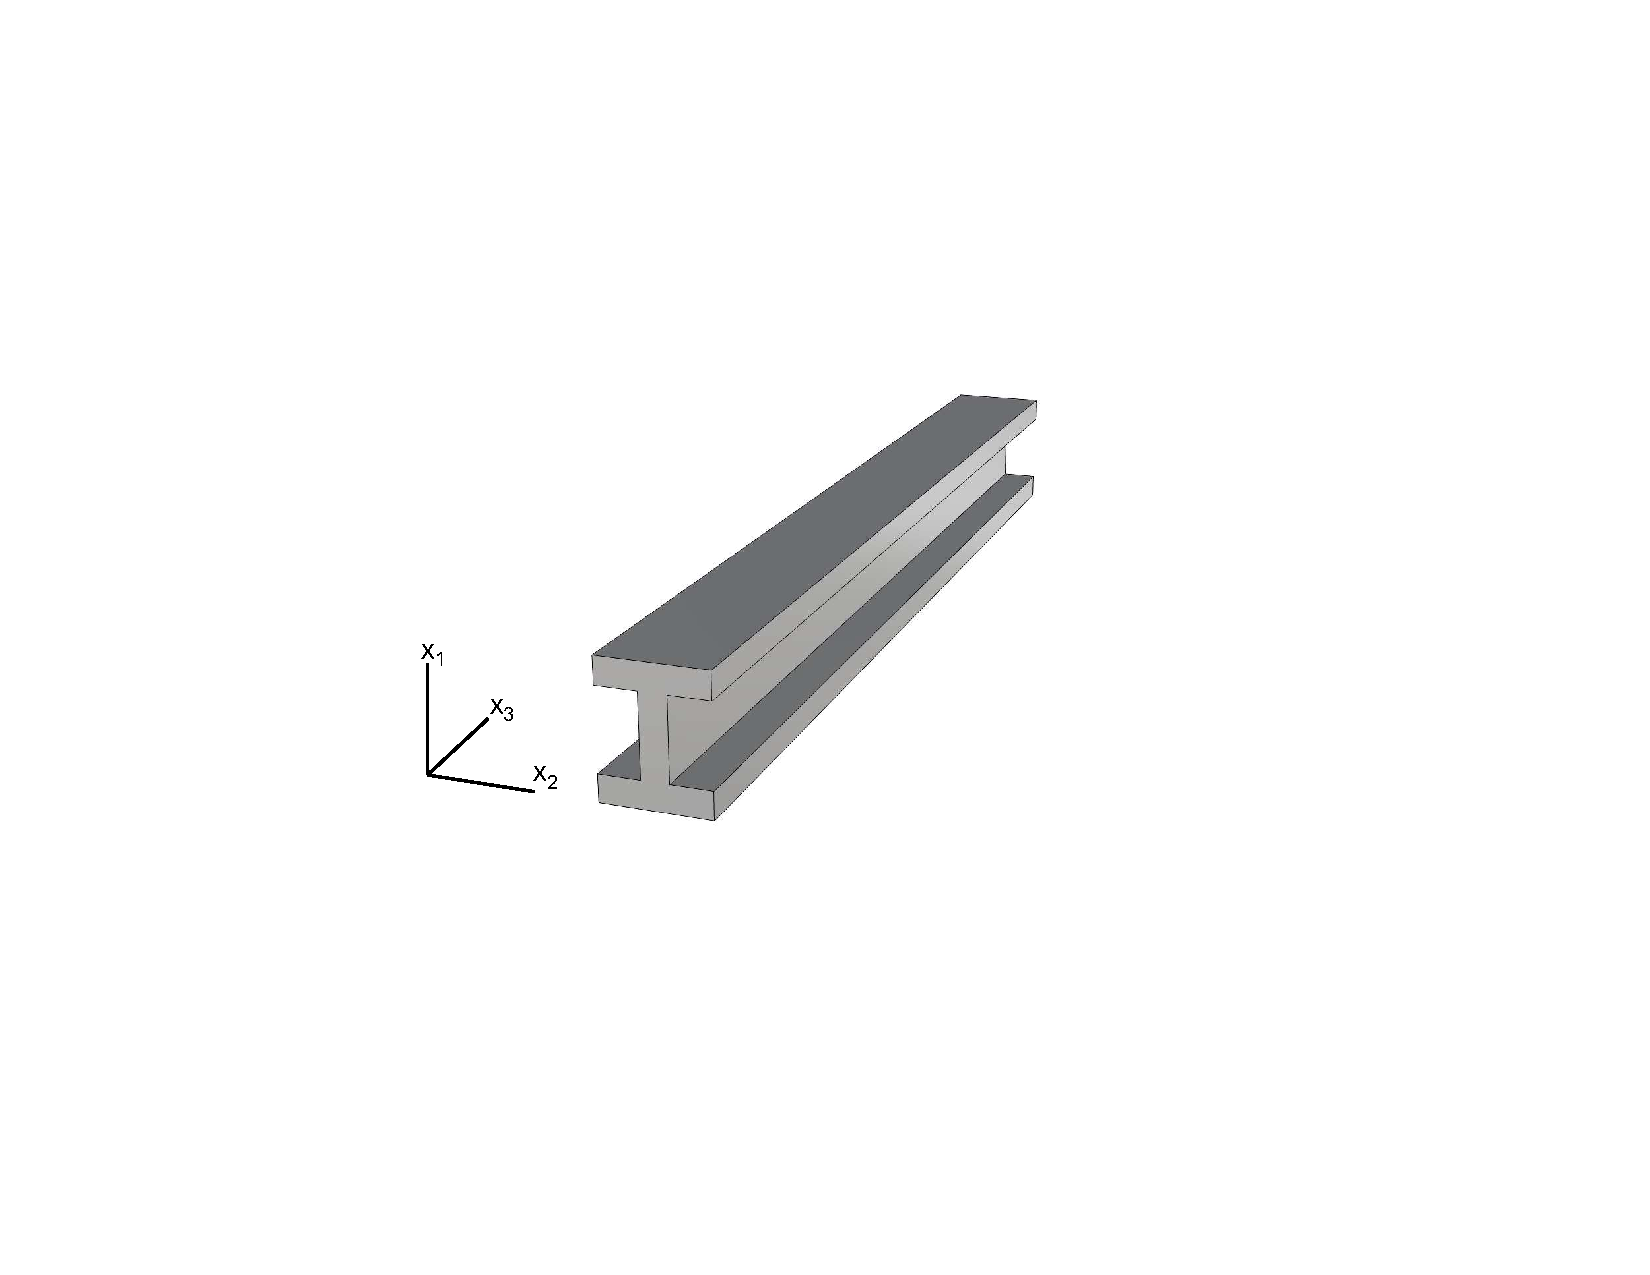
\includegraphics[width=0.25\columnwidth,trim=0cm 3cm 0cm 0cm, clip]{figs/straight.pdf}
%}
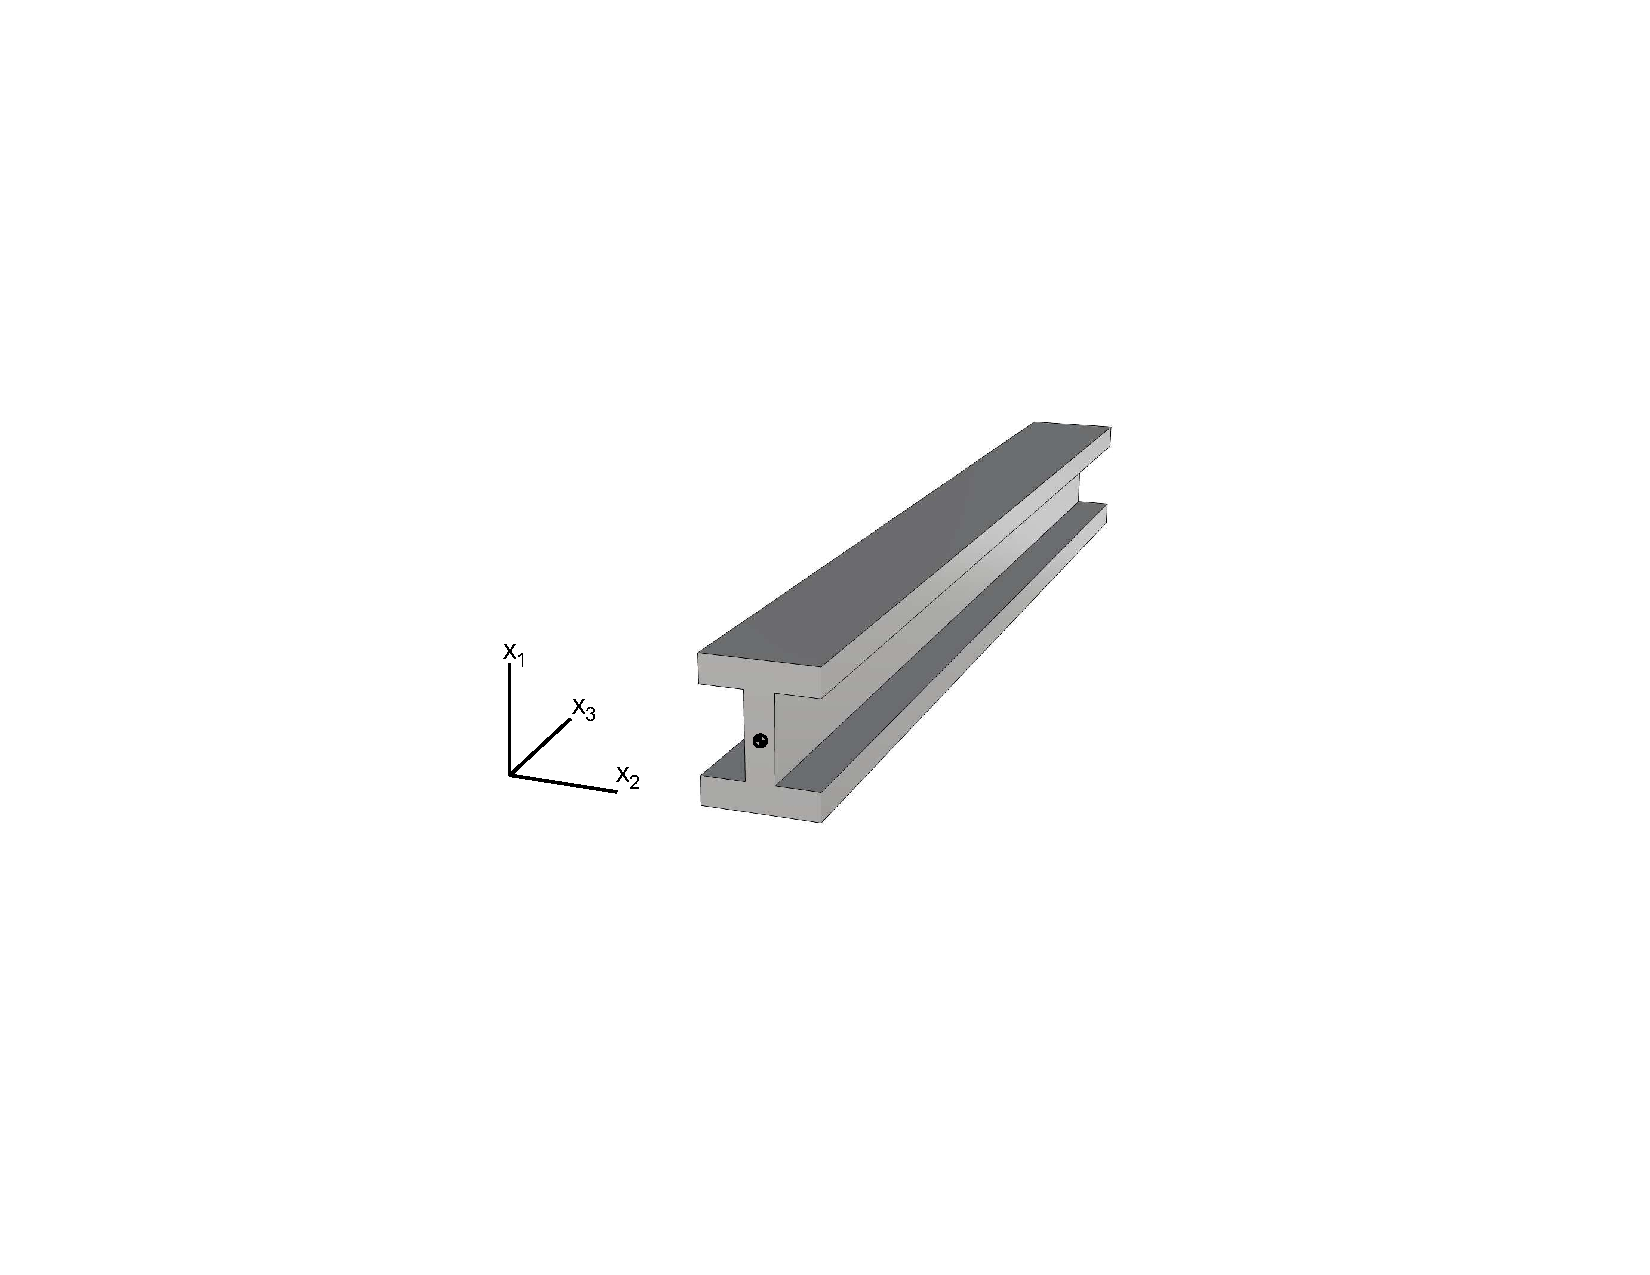
\includegraphics[width=0.7\columnwidth,trim=4cm 7cm 6cm 6cm, clip]{figs/cog.pdf}
\caption{The definition of the beam, with the centroid marked.}
 \label{fig:beam_definition}
\end{figure}


\begin{figure}
\centering
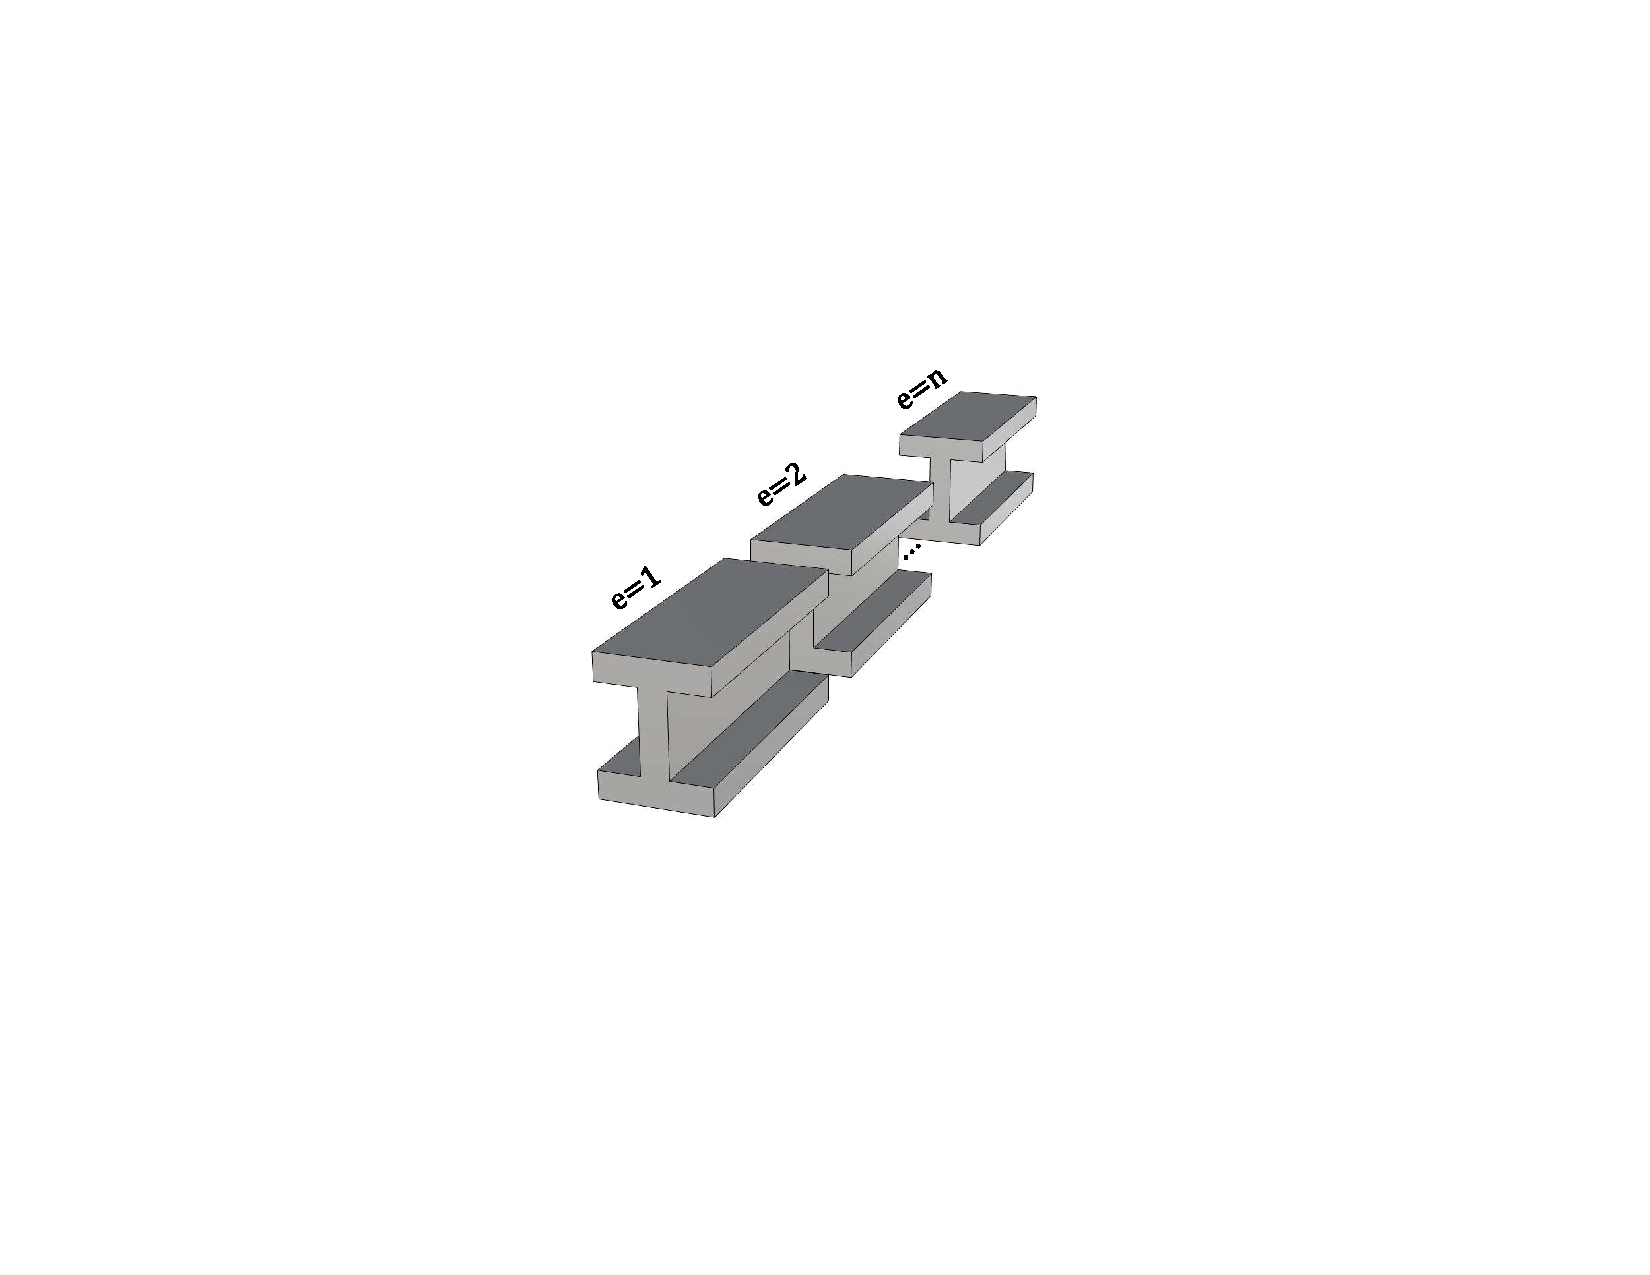
\includegraphics[width=0.7\columnwidth,trim=4cm 7cm 6cm 6cm, clip]{figs/elements.pdf}
\caption{The beam subdivided into n elements}
\label{fig:subdivision}
\end{figure}

%\begin{figure}[htb]
%\centering
%%\subfloat[side view]{
%%	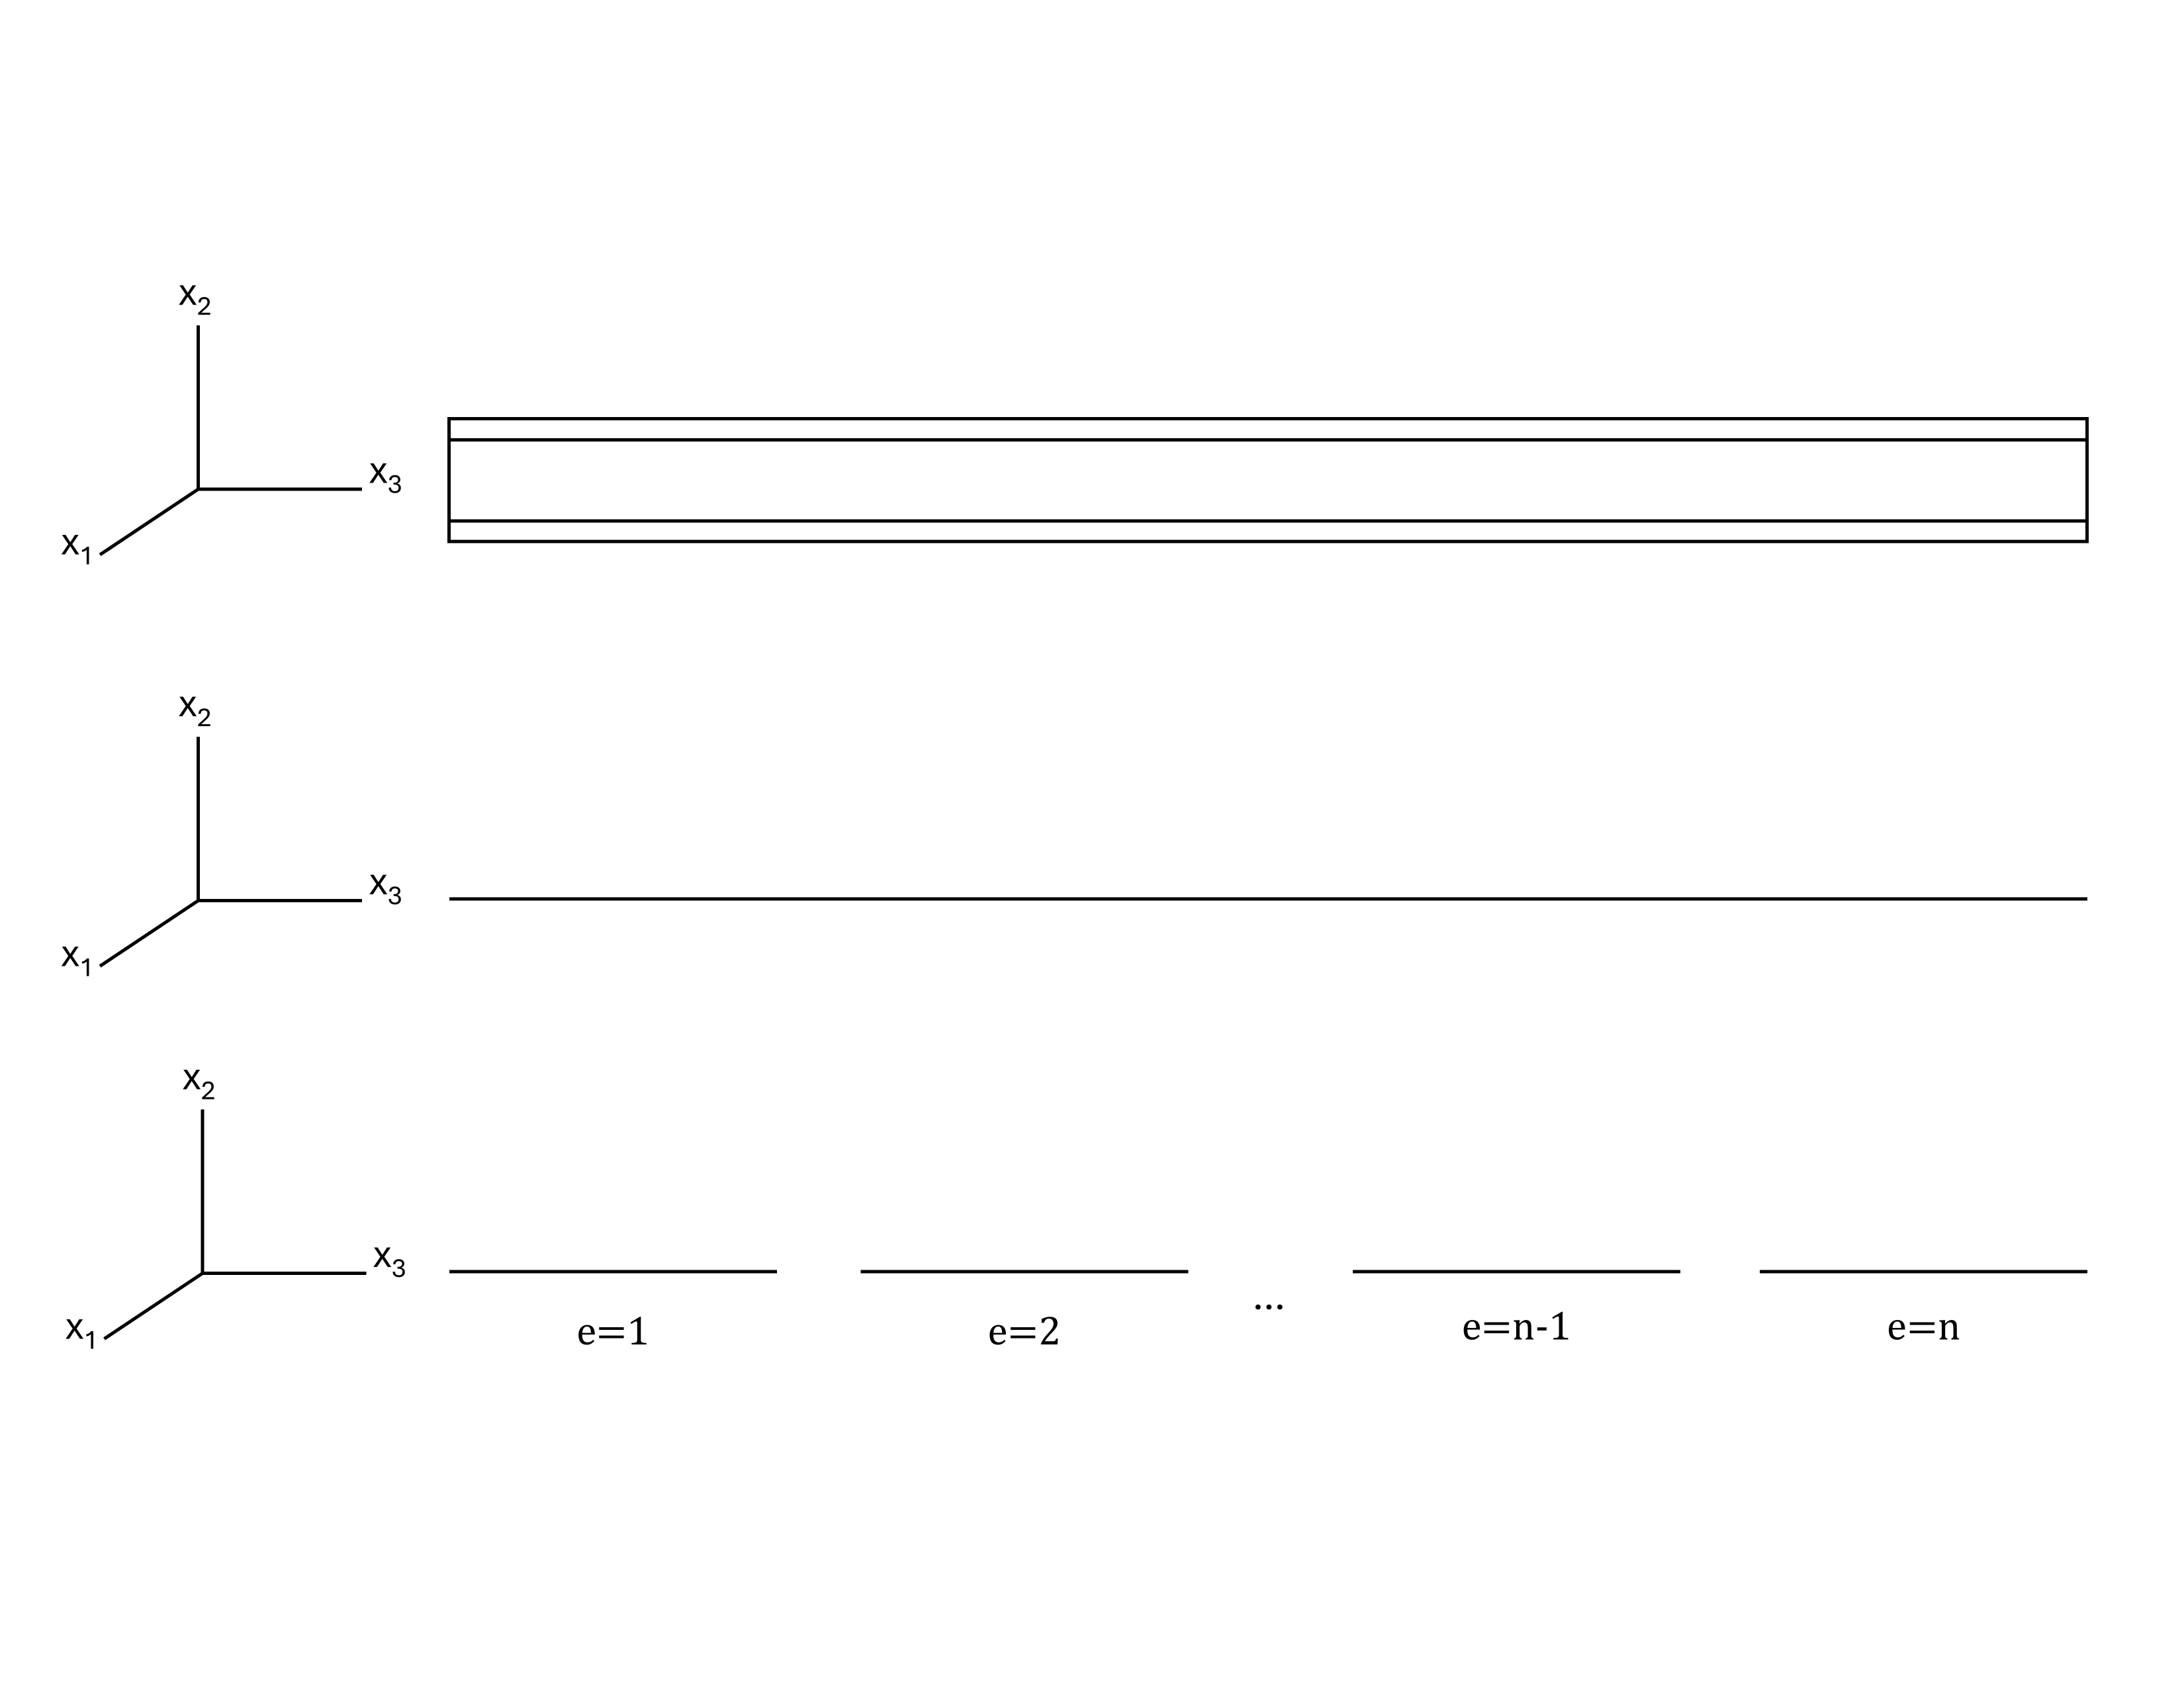
\includegraphics[width=0.7\columnwidth,trim=0cm 13cm 0cm 0cm, clip]{figs/beam_to_elements.png}
%%}
%%\centering
%%\subfloat[isometric view]{
%%	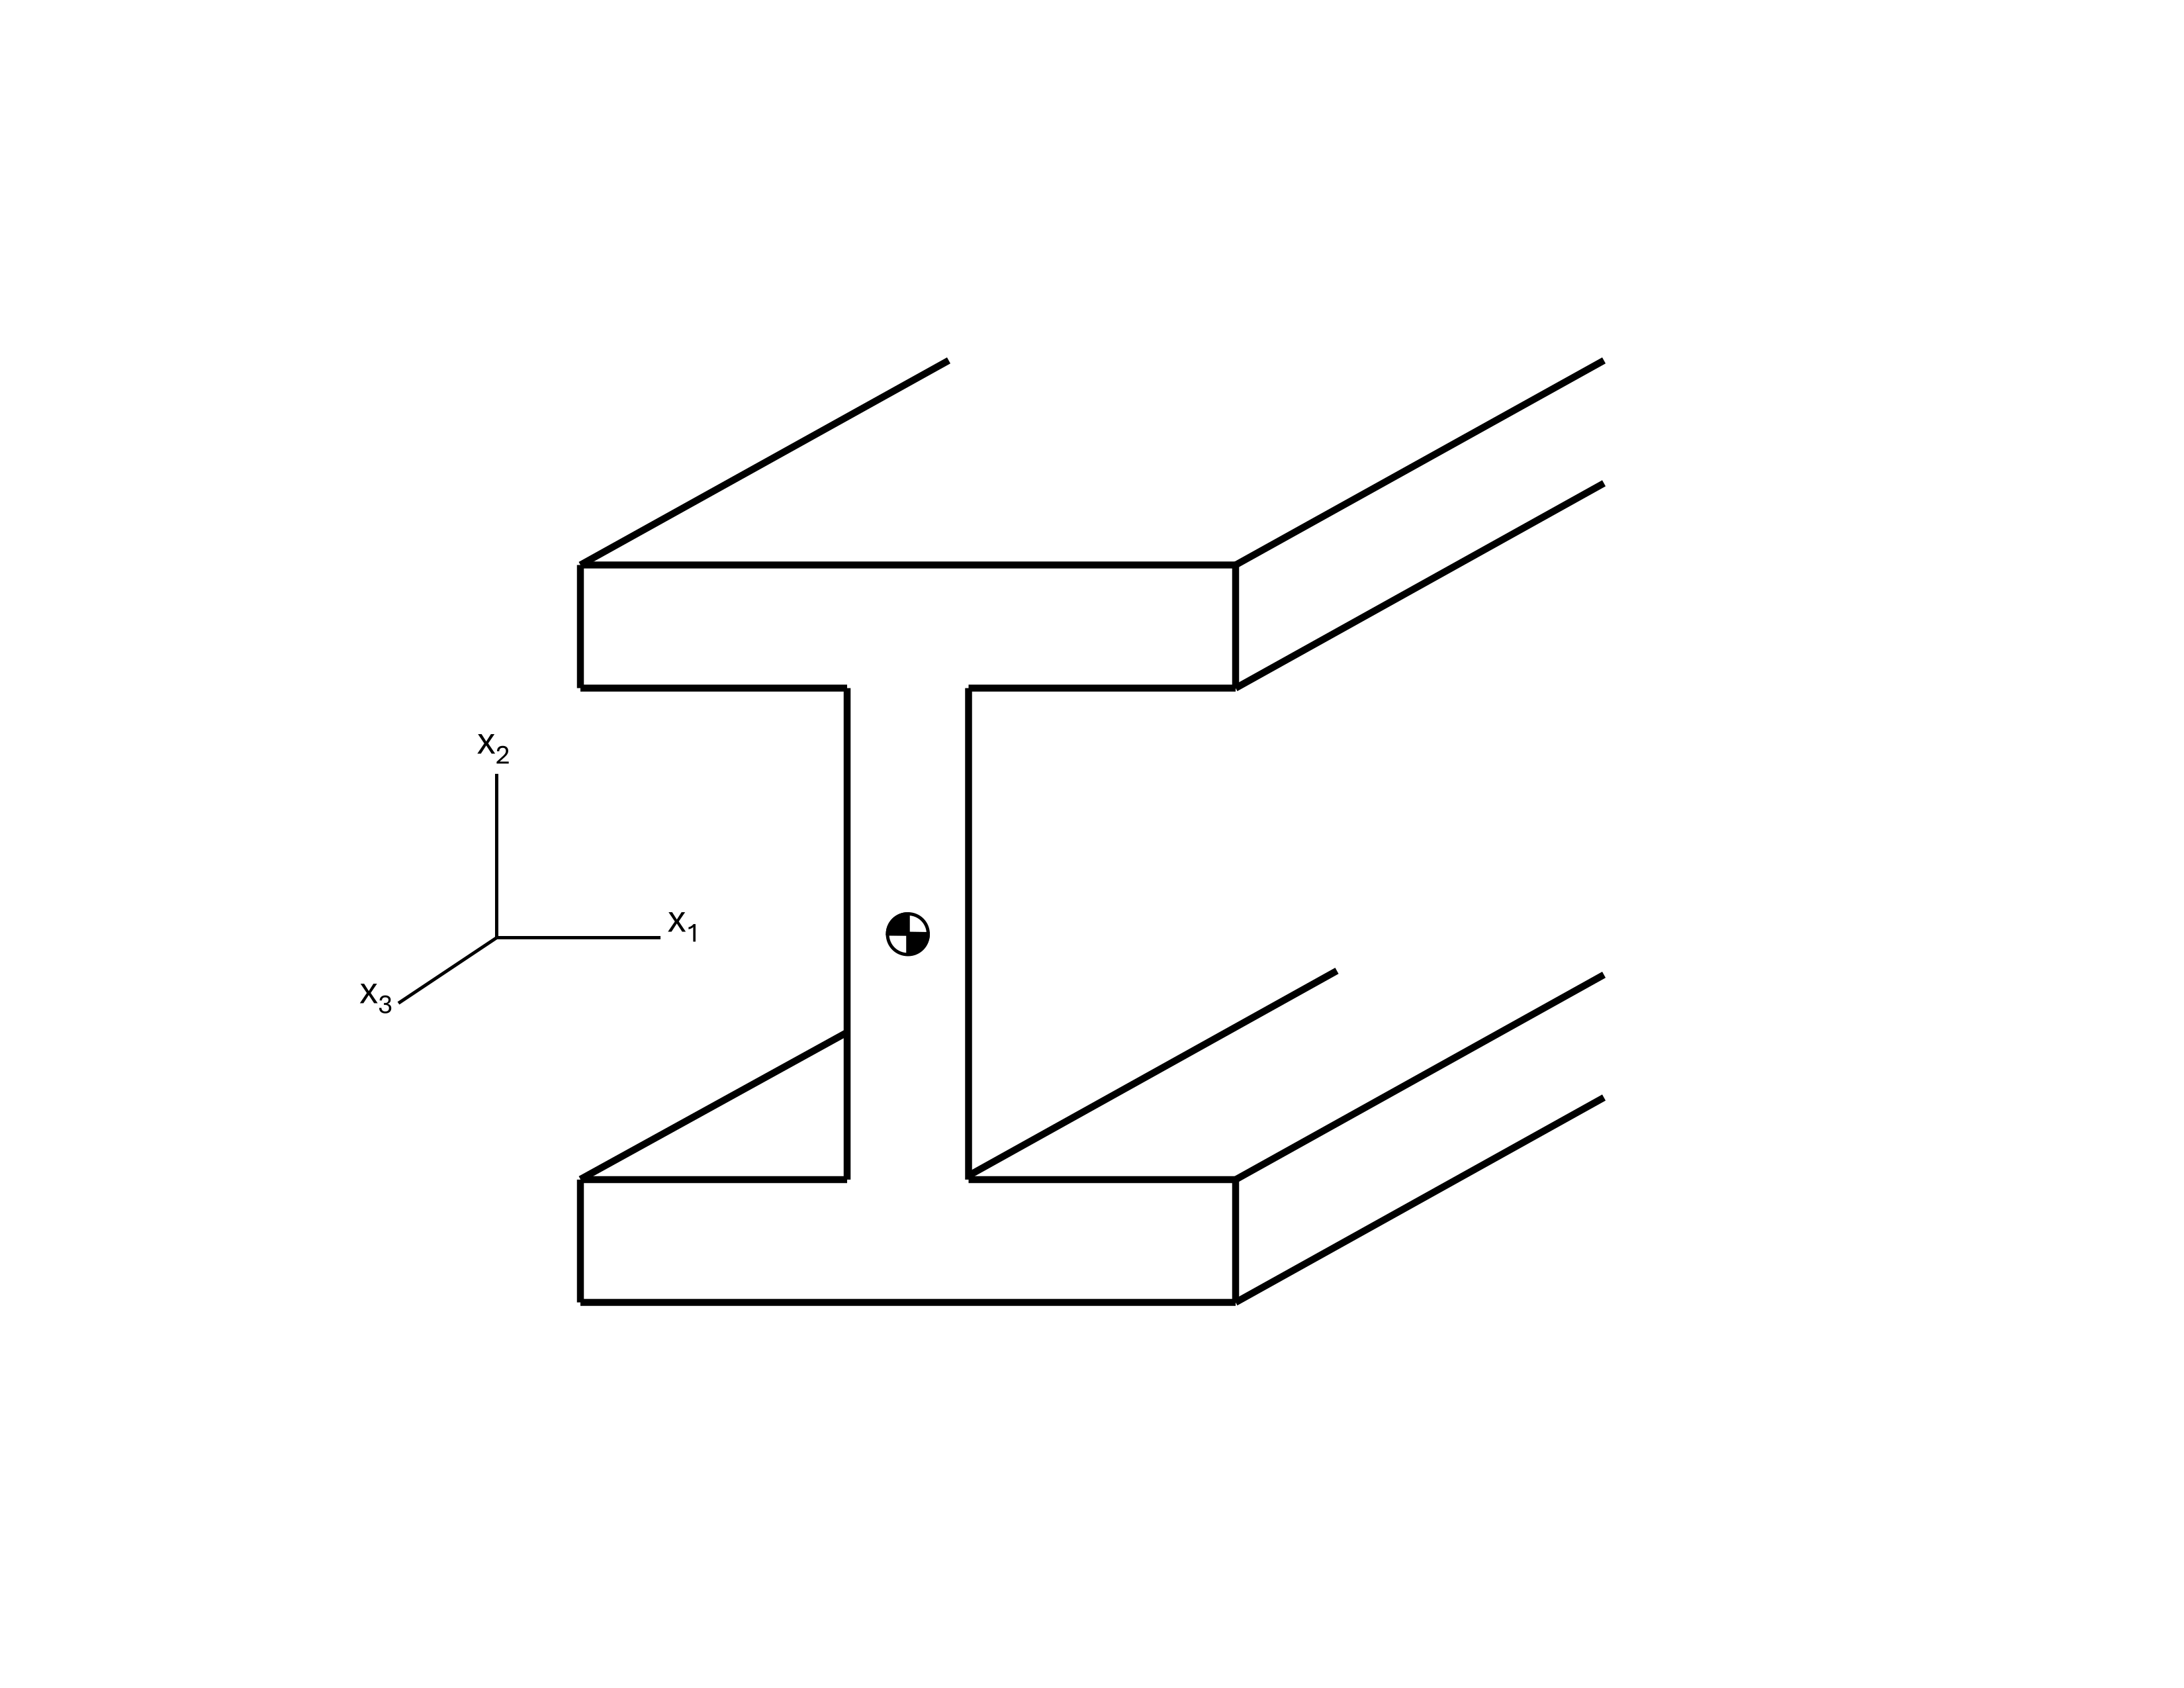
\includegraphics[width=0.25\columnwidth,trim=0cm 3cm 0cm 0cm, clip]{figs/3d_section.png}
%%	\label{fig:iso_view}
%%}
%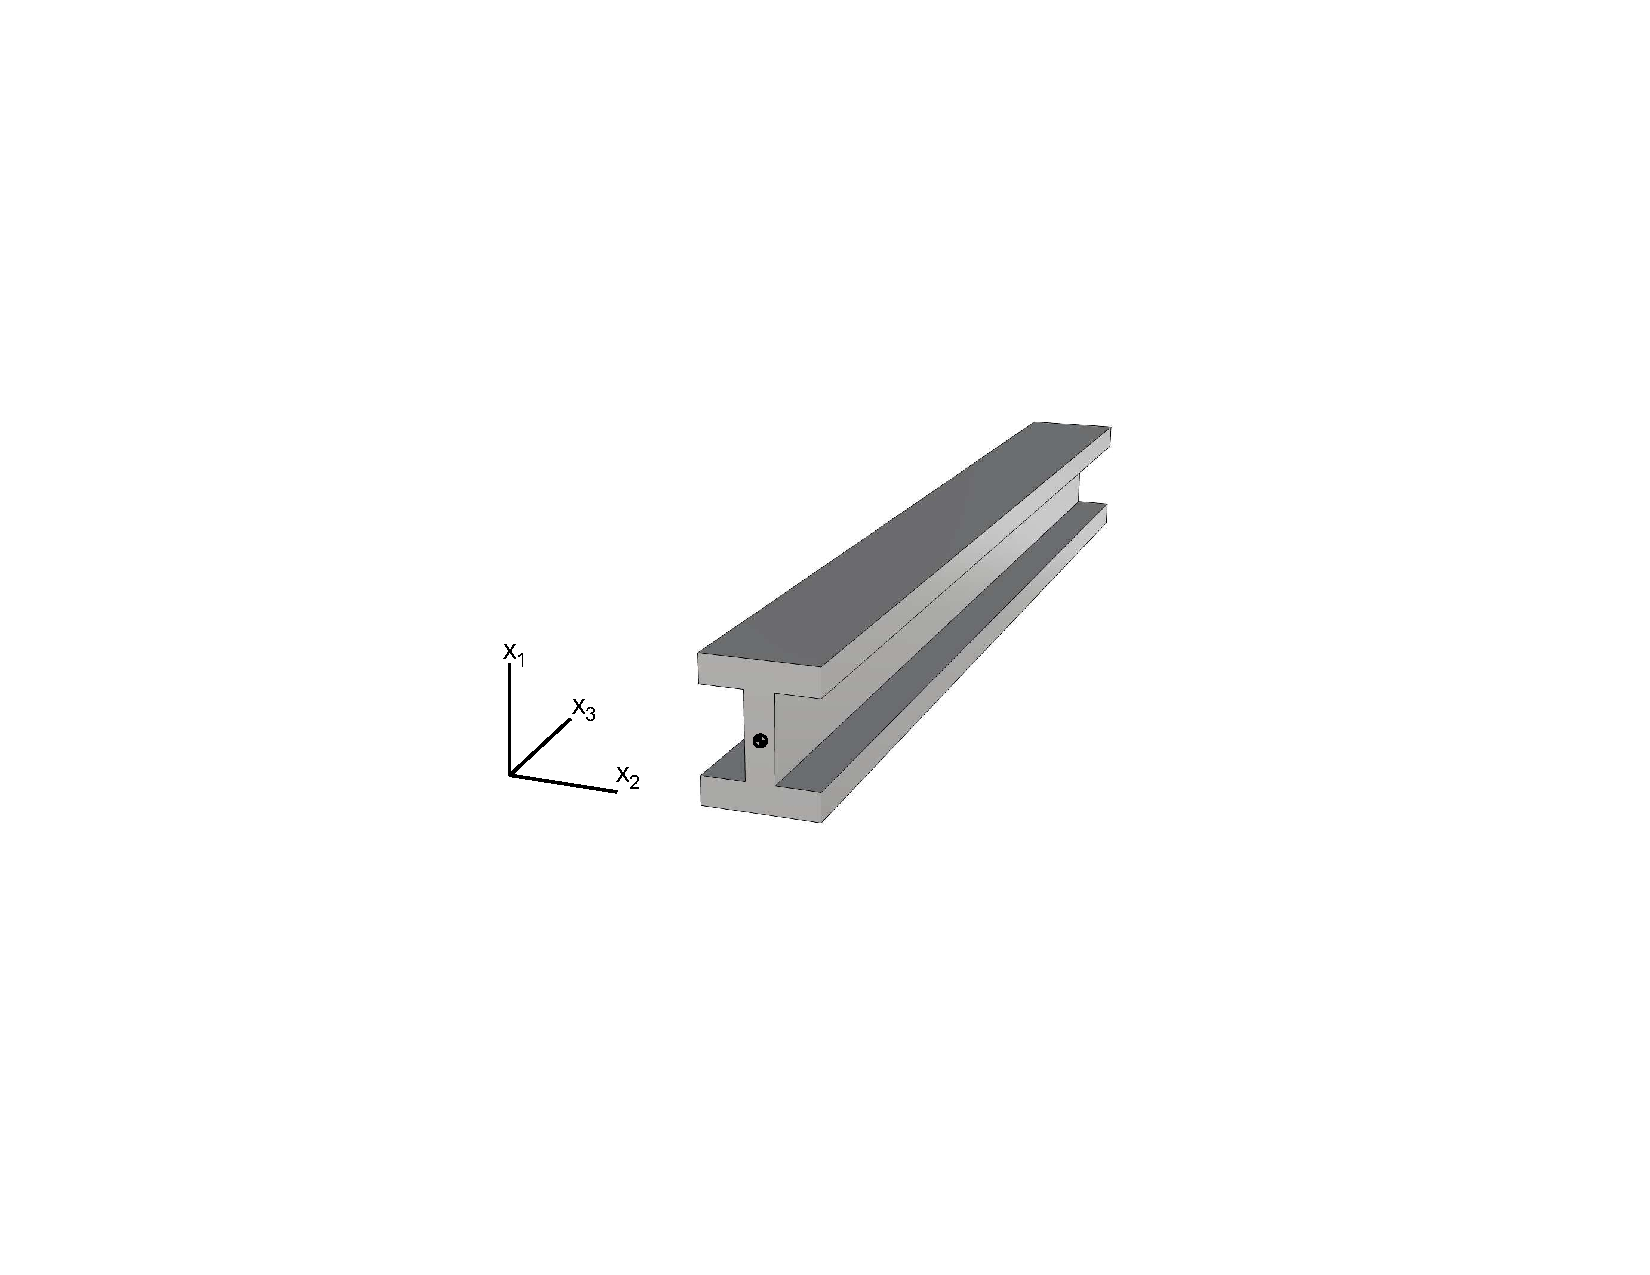
\includegraphics[width=0.7\columnwidth,trim=4cm 7cm 6cm 6cm, clip]{figs/cog.pdf}
%\caption{The centroid of the beam is marked by the center of gravity symbol}
% \label{fig:axis_definition}
%\end{figure}
